\chapter{ಚದುರಂಗದ ಕಾಯಿಗಳ ನಡಿಗೆ ಮಾಯಾಚೌಕಗಳು}

ಮಾಯಾಚೌಕಗಳಿಗೂ ಚದುರಂಗದ ಕಾಯಿಗಳ ನಡಿಗೆಗೂ ಒಂದು ರೀತಿಯ ಸಂಬಂಧ. \hbox{ಸಾಮಾನ್ಯವಾಗಿ 8ನೆ} ಕ್ರಮವರ್ಗದ ಮಾಯಾಚೌಕವನ್ನು ಚದುರಂಗದ ರಾಜ, ಕುದುರೆ ಮೊದ\-ಲಾದ ಕಾಯಿಗಳ ನಡಿಗೆಯಿಂದ ತುಂಬಿಸಿ,ರಚಿಸಲಾಗುತ್ತದೆ. 1 ರಿಂದ 64ರವರೆಗೆ ಸಂಖ್ಯೆ\-ಗಳನ್ನು ಕಾಯಿ ಚಲಿಸುವ ಮನೆಗಳಿಗೆ ತುಂಬಿಸಬೇಕು. ಒಂದು ಬಾರಿ ಹೋದ ಮನೆಗೆ ಮತ್ತೆ ಹೋಗುವಂತಿಲ್ಲ. ಎಲ್ಲ ಮನೆಗಳೂ ತುಂಬಿದ ಮೇಲೆ ಮಾಯಾಚೌಕ ಲಭಿಸುವುದು.

ಕೆಲವು ಉದಾಹರಣೆಗಳನ್ನು ನೋಡೋಣ.

\section*{VII.1. ಚದುರಂಗದ ರಾಜನ ನಡಿಗೆಯ ಮಾಯಾಚೌಕ}

ಮಾಯಾಚೌಕಕ್ಕೂ ಚದುರಂಗದ ರಾಜ ಮತ್ತು ಕುದುರೆಗಳಿಗೂ ಒಂದು ರೀತಿಯ ನಂಟು. ಇವುಗಳನ್ನು ಬಳಸಿ ಆಕರ್ಷಕ ಮಾಯಾಚೌಕ ರಚಿಸಿದ್ದಾರೆ ಮಾಯಾಚೌಕ ತಜ್ಞರು. ನಾವು ಅಂತಹ ಮಾಯಾಚೌಕಗಳನ್ನು ನೋಡಿ ಖುಷಿ ಪಡೋಣ.

ಚದುರಂಗದ ಆಟದಲ್ಲಿ ರಾಜನಿಗೆ ಸೀಮಿತ ನಡಿಗೆ. ಯಾವುದೇ ದಿಕ್ಕಿನಲ್ಲಿಯಾದರೂ \hbox{ಒಂದು ಮನೆ ಸರಿಯಬಹುದು.}

ಈ ಕೆಳಗಿನ ಚಿತ್ರದಲ್ಲಿರುವ ಮಾಯಾಚೌಕದಲ್ಲಿ 1 ಎಂದು ಗುರ್ತಿಸಿರುವ ಮನೆಯಿಂದ ಹೊರಟ ರಾಜ ಒಂದೊಂದೇ ಮನೆ ಚಲಿಸಿ 64 ಮನೆಗಳನ್ನೂ ಮುಟ್ಟುತ್ತಾನೆ. ಈ ಚಲನೆಯ ಮನೆಗಳನ್ನು ಅನುಕ್ರಮವಾಗಿ 2,3,4......63,64 ಸಂಖ್ಯೆಗಳಿಂದ ತುಂಬಿಸಿದೆ. ಈಗ ಸಿದ್ಧ\-ವಾಯಿತು ಮಾಯಾಚೌಕ. $8 \times 8$ ಈ ಚೌಕ 8 ಕ್ರಮವರ್ಗದ ಮಾಯಾಚೌಕ.
\begin{figure}[H]
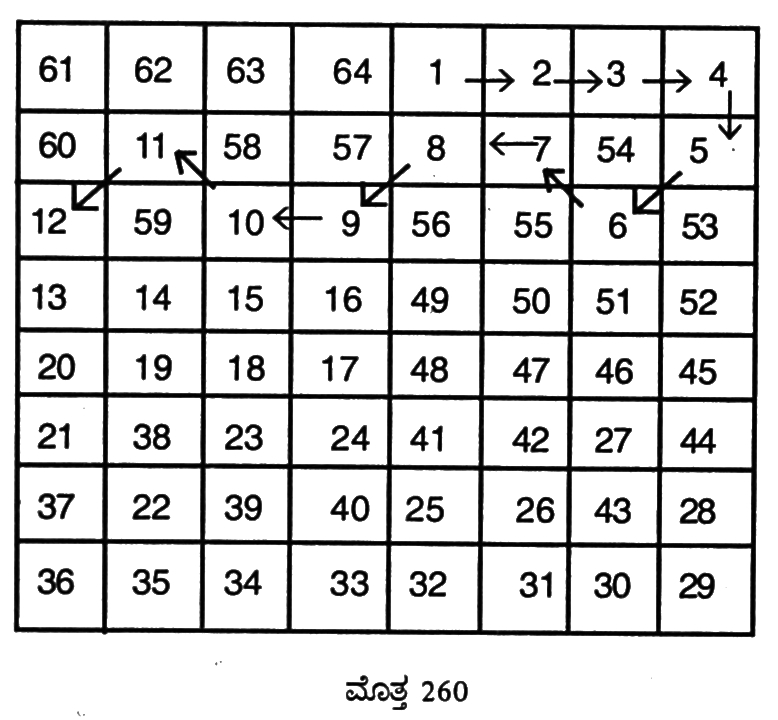
\includegraphics[scale=.8]{src/figures/chap6/fig6-1.jpg}
\end{figure}
\begin{itemize}
	\item ಸೌಕರ್ಯಕ್ಕಾಗಿ ಮೊದಲ ಕೆಲವು ನಡಿಗೆಗಳನ್ನು ಬಾಣದ ಗುರ್ತಿನಿಂದ ಸೂಚಿಸಿದೆ.
	\item ಅಡ್ಡಸಾಲು, ಕಂಭಸಾಲು, ಕರ್ಣಗಳ ಮನೆಗಳಲ್ಲಿರುವ ಸಂಖ್ಯೆಗಳ ಮೊತ್ತ 260
\end{itemize}

\section*{II. 2. ಕುದುರೆ ನಡಿಗೆಯ ಮಾಯಾಚೌಕಗಳು :}

ಚದುರಂಗ ಆಟದಲ್ಲಿ ಕುದುರೆ ನಡಿಗೆಯು ಅತಿ ವಿಶಿಷ್ಟ . ಕುದುರೆಯು ತನ್ನ ಮನೆಯಿಂದ ಅಡ್ಡಲಾಗಿ ಅಥವಾ ಉದ್ದವಾಗಿ 2 ಮನೆ ಚಲಿಸಿ, ನಂತರ ಬಲಕ್ಕೆ ಎಡಕ್ಕೆ, ಕೆಳಕ್ಕೆ ಅಥವಾ ಮೇಲಕ್ಕೆ ಒಂದು ಮನೆ ಚಲಿಸುತ್ತದೆ. ಅಂದರೆ ಸುತ್ತಲಿನ ಎಂಟು ಮನೆಗಳಲ್ಲಿ ಯಾವುದಾದರೂ ಒಂದಕ್ಕೆ ಚಲಿಸಬಹುದು.

ಚಿತ್ರ ನೋಡಿ. ಚದುರಂಗದ ಹಾಸಿನ (Board) \textbf{‘ಎಸ್’} ಗುರುತಿಸಿರುವ ಮನೆಯಲ್ಲಿ \hbox{ಕುದುರೆ ಇದೆಯೆಂದು} ಇಟ್ಟುಕೊಳ್ಳೋಣ. ಅದು ನಾಲ್ಕೂ ಕಡೆಗೆ ಎರಡು ಮನೆ ಚಲಿಸಿ ಅಲ್ಲಿಂದ ಪಕ್ಕಕ್ಕೆ ಒಂದು ಮನೆ ಚಲಿಸಬಲ್ಲದು. ಹೀಗಾಗಿ $‘\bullet ’$ ಗುರುತು ಮಾಡಿರುವ 8 ಮನೆಗಳಲ್ಲಿ ಒಂದಕ್ಕೆ ಚಲಿಸಬಲ್ಲದು. ಬಾಣದ ಗುರುತು ಚಲನೆಯ ದಿಕ್ಕನ್ನು ಸೂಚಿಸುತ್ತದೆ.
\begin{figure}[H]
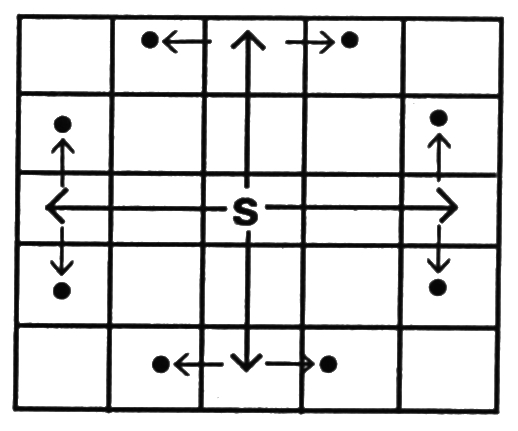
\includegraphics[scale=1.2]{src/figures/chap6/fig6-2.jpg}
\end{figure}

ಕುದುರೆಯ ನಡಿಗೆಯನ್ನನುಸರಿಸಿ ಮನೆಗಳನ್ನು 1,2,3,......64ವರೆಗೆ ತುಂಬಿಸಿ $8 \times 8$ ಮಾಯಾಚೌಕ ರಚಿಸುವುದು ಗಣಿತಜ್ಞರಿಗೆ ಮುದ ತರುವಂತಹದು. ಇಂತಹ ಕೆಲವು ಮಾಯಾಚೌಕಗಳನ್ನು ಪರಿಶೀಲಿಸೋಣ.
\begin{itemize}
	\item $8 \times 8$ ಮಾಯಾಚೌಕ 1 ರಿಂದ 64 ವರೆಗೆ ಕ್ರಮಾಗತ ಸಂಖ್ಯೆ ಬಳಸಿದೆ.
	\item ಚದುರಂಗದ ಕುದುರೆ ನಡಿಗೆ ಕ್ರಮದಲ್ಲಿ ಮನೆಗಳನ್ನು ತುಂಬಿಸಿದೆ.
	\item ಅಡ್ಡಸಾಲು, ಕಂಭಸಾಲು ಸಂಖ್ಯೆಗಳ ಮೊತ್ತ 260
	\item ಕರ್ಣಗಳ ಸಂಖ್ಯೆಗಳ ಮೊತ್ತ 260 ಆಗುವುದಿಲ್ಲ.
	\begin{figure}[H]
	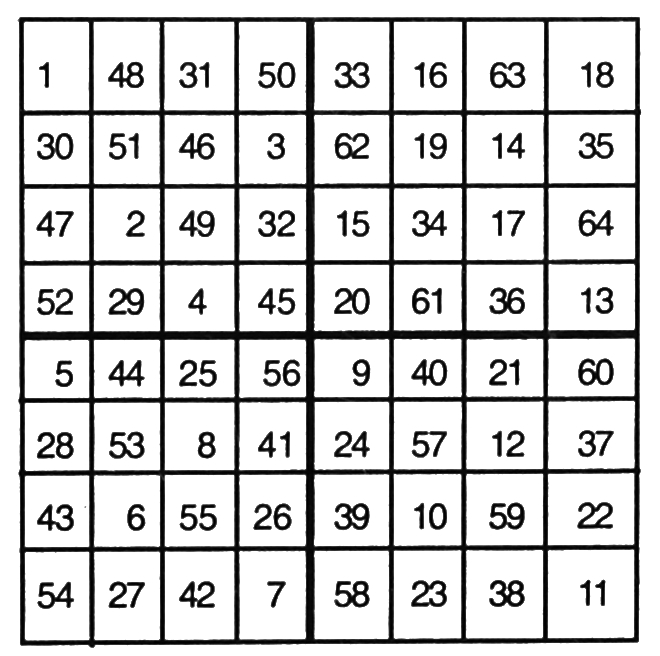
\includegraphics[scale=1.3]{src/figures/chap6/fig6-3.jpg}
	\end{figure}
	\item $8 \times 8$ ಚೌಕವನ್ನು $4 \times 4$ರ ನಾಲ್ಕು ಚೌಕಗಳಾಗಿ ವಿಭಾಗಿಸಿದರೆ ಅವು ಕುದುರೆ ನಡಿಗೆ ಮಾಯಾಚೌಕಗಳೇ (ಕರ್ಣ ಹೊರತು ಪಡಿಸಿ)
	\item ಕಂಭಸಾಲು, ಅಡ್ಡಸಾಲುಗಳಲ್ಲಿ $2 \times 2$ ಚೌಕಗಳ ಸಂಖ್ಯೆಗಳ ಮೊತ್ತ 130.

	ಉದಾ: (1+48+30+51),(49+32+4+45), ಇತ್ಯಾದಿ.

	ಲಿಯೋನಾರ್ಡ್ ಆಯ್ಲರ್ (1707-1783) ರಚಿಸಿದ್ದು
\end{itemize}

\medskip
\textbf{VI. 3.} ಕುದುರೆ ನಡಿಗೆಯ ಮಾಯಾಚೌಕಗಳಲ್ಲಿ ಗಣಿತಜ್ಞರು ಬಗೆಬಗೆಯ ಸಂಖ್ಯಾ \linebreak ಜೋಡಣೆಯನ್ನು ಸಾಧಿಸಿದ್ದಾರೆ. ಅವುಗಳಲ್ಲಿ ಏನಾದರೊಂದು ವಿಶೇಷತೆ ಇರುವುದು \linebreak ಸಾಮಾನ್ಯ. ಇಂತಹ ಒಂದು ಮಾಯಾಚೌಕವನ್ನು ಮೈಸೂರಿನ ಜಗನ್ಮೋಹನ ಅರಮನೆಯ ಕಲಾಗ್ಯಾಲರಿಯಲ್ಲಿ ನೋಡಬಹುದು. ಇದಕ್ಕೆ  \textbf{‘‘ತಾರೈಕಾಶ್ವಗತಿ ಮಾಯಾಚೌಕ’’} ಎಂದು ಹೆಸರಿಸ\-ಲಾಗಿದೆ. ಇದು \textbf{‘‘ಅಶ್ವಗತಿ’’} (ಕುದುರೆ ನಡಿಗೆ) ಯೂ ಹೌದು. ಇದರಲ್ಲಿ ನಕ್ಷತ್ರ ಆಕೃತಿಗಳನ್ನೂ ಕಾಣಬಹುದು. ಇದೊಂದು ತೆರೆದ ಮಾಯಾಚೌಕ. ಅಂದರೆ ಪ್ರಾರಂಭದ ಮನೆ (1) ಮತ್ತು ಕೊನೆಯ ಮನೆ (64) ಇವುಗಳು ಕುದುರೆ ನಡಿಗೆಯ ಒಂದು ನಡಿಗೆ ಅಂತರದಲ್ಲಿಲ್ಲ. ಈ ಚೌಕವನ್ನು ಕೆಳಗೆ ಕೊಟ್ಟಿದೆ. ಮೊತ್ತ : 260
\begin{itemize}
	\item ಸಂಖ್ಯೆಗಳನ್ನು ಚದುರಂಗದ ಕುದುರೆ ನಡಿಗೆಯಂತೆ ತುಂಬಲಾಗಿದೆ.
	\item ಪ್ರತಿ ಅಡ್ಡಸಾಲು, ಕಂಭಸಾಲು, ಸಂಖ್ಯೆಗಳ ಮೊತ್ತ 260. ಕರ್ಣಸಾಲಿನದು ಬೇರೆ. ಇದೊಂದು ಊನ ಮಾಯಾಚೌಕ.
	\begin{figure}[H]
	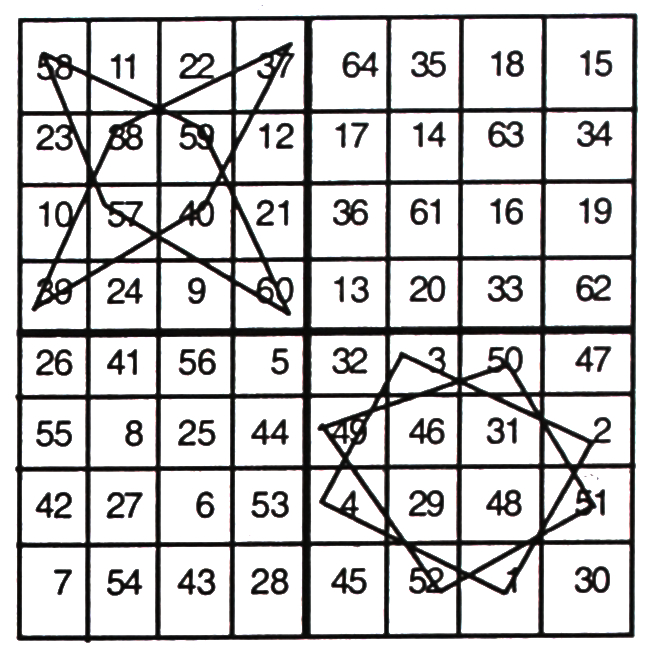
\includegraphics[scale=1.2]{src/figures/chap6/fig6-4.jpg}
	\end{figure}
	\item ಎರಡೆರಡು ಅಡ್ಡಸಾಲುಗಳ ಅಥವಾ ಎರಡೆರಡು ಕಂಭಸಾಲುಗಳಲ್ಲಿ $2 \times 2$ (ನಾಲ್ಕು) ಚೌಕಗಳ ಮೊತ್ತ 130.

	$58+11+23+38=130; 64+35+17+14=13-0,$

	$26+41+55+8= 130; 48+51+1+30=130,$
	\item ಚೌಕವನ್ನು $4 \times 4$ ರ ನಾಲ್ಕು ಸಮಭಾಗಗಳಾಗಿ ವಿಭಾಗಿಸಿ. ಅವುಗಳಲ್ಲಿ ಕ್ರಮಾಗತ ಸಂಖ್ಯೆ\-ಗಳನ್ನು ಸರಳರೇಖೆಗಳಿಂದ ಸೇರಿಸಿ. ನಕ್ಷತ್ರ ಆಕೃತಿ ಬರುತ್ತದೆ. ಎರಡು ಚೌಕ\-ಗಳಲ್ಲಿ ಬೇರೆ ಬೇರೆ ರೀತಿಯ ನಕ್ಷತ್ರ ಆಕೃತಿ ರಚಿಸಿ ತೋರಿಸಿದೆ.
\end{itemize}

\medskip
\textbf{VII. 4.} ಚದುರಂಗದ ಕುದುರೆ ನಡಿಗೆಯ ಮಾಯಾಚೌಕಗಳಲ್ಲಿ ಎರಡು ಮುಖ್ಯ ಬಗೆಯವುಗಳನ್ನು ಗುರುತಿಸಲಾಗಿದೆ. ಪ್ರಾರಂಭದ ಮನೆಯೂ ಮತ್ತು ಕೊನೆಯ ಮನೆಯೂ \hbox{ಒಂದು ಕುದುರೆ} ನಡಿಗೆಯ ಅಂತರದಲ್ಲಿದ್ದರೆ, ಅಂತಹ ಚೌಕಗಳನ್ನು  \textbf{‘‘ಮುಚ್ಚಿದ’’} ಅಥವಾ \textbf{‘‘ಪುನಃ ಪ್ರವೇಶ’’} ಚೌಕಗಳೆಂದು ಹೇಳಲಾಗಿದೆ. ಹಾಗಿಲ್ಲದೇ ಮೊದಲ ಮತ್ತು ಕೊನೆಯ ಮನೆಗಳು ದೂರವಾಗಿದ್ದರೆ ಅವು \textbf{‘‘ತೆರೆದ’’} ಚೌಕಗಳು.

$8 \times 8$ ರ ಕುದುರೆ ನಡಿಗೆಯ ಇನ್ನೂ ಕೆಲವು ಚೌಕಗಳನ್ನು ನೋಡೋಣ.
\begin{itemize}
	\item ಊನ ಮಾಯಾಚೌಕ, ಕರ್ಣಗಳ ಮೊತ್ತ ಬೇರೆ.
	\item ಮೊತ್ತ 260
	\item \textbf{‘‘ಮುಚ್ಚಿದ’’ ‘‘ಮಾಯಾಚೌಕ’’}
	\item 1862 ರಲ್ಲಿ ಸಿ. ಎಫ್. ಜೇನಿಷ್ ಎಂಬಾತನು ರಚಿಸಿದ್ದು
	\begin{figure}[H]
	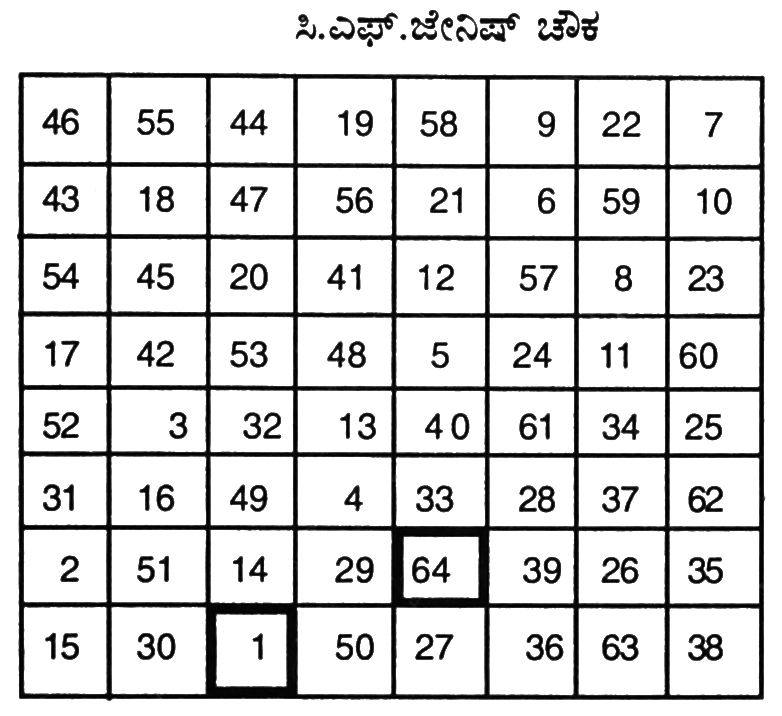
\includegraphics[scale=.9]{src/figures/chap6/fig6-5.jpg}
	\end{figure}
	\begin{figure}[H]
	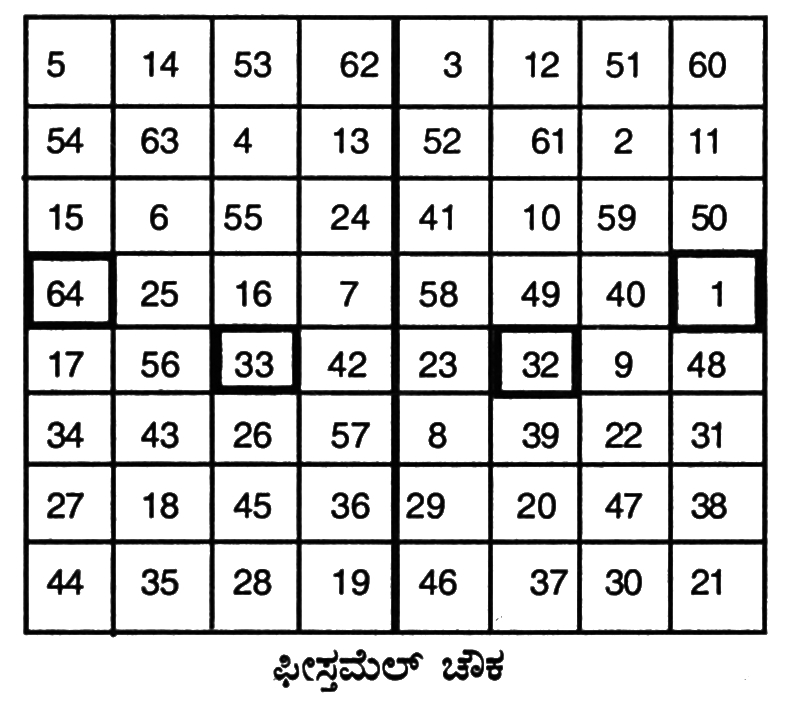
\includegraphics[scale=.9]{src/figures/chap6/fig6-6.jpg}
	\end{figure}
	\item ಅಡ್ಡಸಾಲು, ಕಂಭಸಾಲು, ಕರ್ಣಸಾಲುಗಳಲ್ಲಿನ ಸಂಖ್ಯೆಗಳ ಮೊತ್ತ 260
	\item 1ರಿಂದ 32 ವರೆಗೆ ಕುದುರೆ ನಡಿಗೆಯಲ್ಲಿ ಸಂಖ್ಯೆಗಳನ್ನು ತುಂಬಿಸಿದೆ.
	\item 32ರ ನಂತರ ಎಡಗಡೆಗೆ 3 ಮನೆ ಆನೆ ನಡಿಗೆಯಲ್ಲಿ 33ಕ್ಕೆ
	\item 33ರಿಂದ 64ವರೆಗೆ ಮತ್ತೆ ಕುದುರೆ ನಡಿಗೆಯಲ್ಲಿದೆ.
	\item ಫೀಸ್ತಮೆಲ್ ಎಂಬಾತ ರಚಿಸಿದುದು
	\item ಉದ್ದುದ್ದಕ್ಕೆ ಭಾಗವಾಗಿ ಸೀಳಿದಾಗ, ದರ್ಪಣ ಪ್ರತಿಬಿಂಬ ಸ್ಥಾನಗಳಲ್ಲಿ ಬರುವ ಸಂಖ್ಯೆಗಳ ಮೊತ್ತ 65. (ಉದಾ: 62+3, 53+12, 14+51, 5+60 ಇತ್ಯಾದಿ)
\end{itemize}

\section*{VII. 5. ಇನ್ನೊಂದು ಕುದುರೆ ನಡಿಗೆಯ ಮಾಯಾಚೌಕ ಪರಿಶೀಲಿಸೋಣ}

\begin{itemize}
	\item ಊನ ಮಾಯಾಚೌಕ. ಅಡ್ಡಸಾಲು ಕಂಭಸಾಲುಗಳಲ್ಲಿನ ಸಂಖ್ಯೆಗಳ ಮೊತ್ತ 260 ಕರ್ಣಗಳ ಸಂಖ್ಯೆಗಳ ಮೊತ್ತ ಬೇರೆ.
	\item ಚದುರಂಗ ಕುದುರೆ ನಡಿಗೆಯಲ್ಲಿ ಸಂಖ್ಯೆಗಳನ್ನು ತುಂಬಿಸಿದೆ. ‘‘ಮುಚ್ಚಿದ’’ ಮಾಯಾಚೌಕ.
	\item ವೆನ್ಸೆಲೀಡ್ ಎಂಬಾತ ರಚಿಸಿದುದು
	\item ಕರ್ಣಗಳಿಗೆ ಅನ್ವಯಿಸುವಂತೆ ಓರೆ (Skew) ಸಮಮಿತಿ ಕಂಡು ಬರುತ್ತದೆ.

	ಕೇಂದ್ರದಿಂದ ಅನುರೂಪ ಮನೆಗಳಲ್ಲಿನ ಸಂಖ್ಯೆಗಳ ವ್ಯತ್ಯಾಸ 32.

	(ಉದಾ : 52-20, 50-18, 35-3, 45-13, 56-24, 55-23 ಇತ್ಯಾದಿ)
	\begin{figure}[H]
	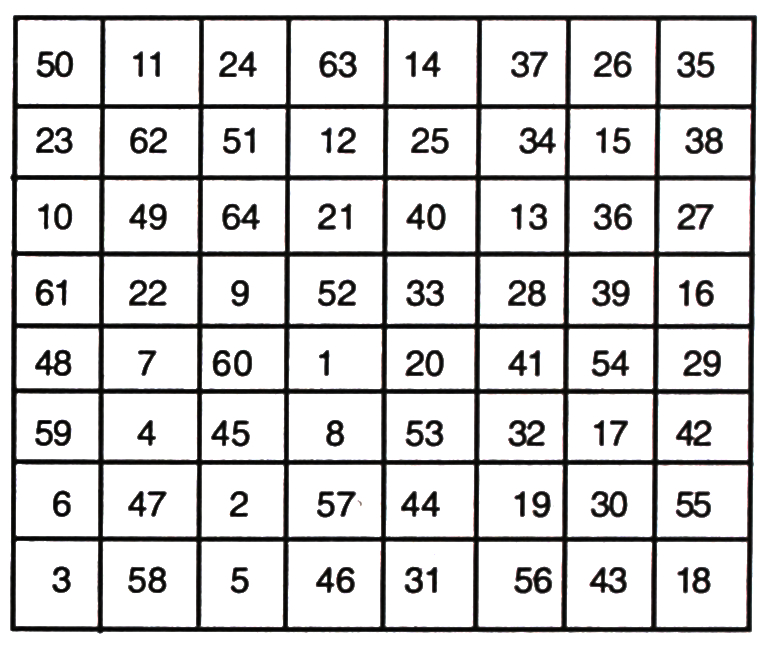
\includegraphics{src/figures/chap6/fig6-7.jpg}
	\end{figure}
\end{itemize}

\section*{VII. 6. ಕುದುರೆ ನಡಿಗೆಯ ಚೌಕಗಳು (Knight Tours)}

ಕುದುರೆ ನಡಿಗೆಯ ಮನೆಗಳಿಗೆ ಕ್ರಮವಾಗಿ ಸಂಖ್ಯೆಗಳನ್ನು ಕೊಟ್ಟು ಮಾಯಾಚೌಕ ರಚಿಸುವ ಹಲವು ವಿಧಗಳನ್ನು ನೋಡಿದೆವು. ಆದರೆ ಗಣಿತಜ್ಞರ ಲೋಕವೇ ಬೇರೆ. ಚೌಕಗಳಲ್ಲಿ ಕುದುರೆ ನಡಿಗೆಯ ಮೂಲಕ ಎಲ್ಲಾ ಮನೆಗಳನ್ನು ಸಂಪರ್ಕಿಸುವುದು. ನಡಿಗೆ ಕ್ರಮದಲ್ಲಿ ವ್ಯತ್ಯಯ ಬರಬಾರದು, ಹೋದ ಮನೆಗೆ ಮತ್ತೆ ಹೋಗಬಾರದು. ಈ ನಿರ್ಬಂಧಗಳಿಗೊಳಪಟ್ಟು ಕೆಲವರು ತಮ್ಮದೇ ವಿಶಿಷ್ಟ ರೀತಿಯಲ್ಲಿ ಚೌಕಗಳನ್ನು ರಚಿಸಿದ್ದಾರೆ. ಇವು ಮಾಯಾಚೌಕಗಳಲ್ಲ. ಅಡ್ಡಸಾಲು, ಕಂಭಸಾಲು, ಕರ್ಣಗಳ ಸಂಖ್ಯೆಗಳ ಮೊತ್ತ ಬೇರೆ ಬೇರೆ. ಇದು ಚದುರಂಗ ಹಾಸಿನ ಎಲ್ಲಾ ಮನೆಗಳಿಗೂ ಕುದುರೆಯ ಪ್ರವಾಸ ಮಾತ್ರ. ಇಂತಹ ಕೆಲವು ಉದಾಹರಣೆಗಳನ್ನು \break ನೋಡೋಣ.

\begin{itemize}
	\item ಡಿ ಮಾವ್ರ್ (1667-1754) ಫ್ರೆಂಚ್ ಗಣಿತಜ್ಞ. ಇಂಗ್ಲೆಂಡಿನಲ್ಲಿ ನೆಲೆಸಿದ. ಸಂಭವ\-ನೀಯತೆಯ ಮೇಲೆ ಪುಸ್ತಕ ಬರೆದ.ಇವನು ರಚಿಸಿದ ಚೌಕ.
	\item $8 \times 8$ರ ಚೌಕವನ್ನು ಕುದುರೆ ನಡಿಗೆಯಲ್ಲಿ ತುಂಬಿಸಿದೆ. ಮಾಯಾಚೌಕವಲ್ಲ.
	\item ತೆರೆದ ಚೌಕ. 1 ಮತ್ತು 64 ಕುದುರೆ ನಡಿಗೆಯಲ್ಲಿ ಇಲ್ಲ.
	\begin{figure}[H]
	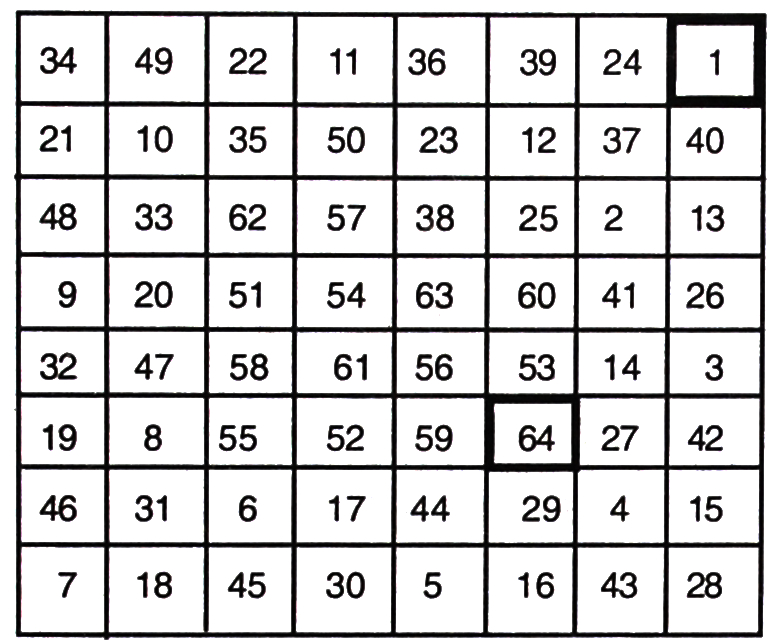
\includegraphics[scale=.9]{src/figures/chap6/fig6-8.jpg}
	\end{figure}

	\item ಲೆಜಾಂಡ್ರ್ ಆಡ್ರಿಯನ್ ಮೇರೀ (1752-1833) ಫ್ರೆಂಚ್ ಗಣಿತಜ್ಞ. ಸಂಖ್ಯಾಗಣಿತದಲ್ಲಿ ಹೆಸರು ಮಾಡಿದವನು. ಇವನು ರಚಿಸಿದ ಚೌಕ.
	\item $8 \times 8$ರ ಚೌಕವನ್ನು ಕುದುರೆ ನಡಿಗೆಯಲ್ಲಿ ತುಂಬಿಸಿದೆ. ಮಾಯಾಚೌಕವಲ್ಲ.
	\item \textbf{‘‘ಮುಚ್ಚಿದ’’} ಅಥವಾ  \textbf{‘‘ಪುನಃ ಪ್ರವೇಶ’’} ಚೌಕ. 1 ಮತ್ತು 64 ಕುದುರೆ ನಡಿಗೆಯಲ್ಲಿ ಒಂದು ನಡಿಗೆಯಲ್ಲಿವೆ.
	\begin{figure}[H]
	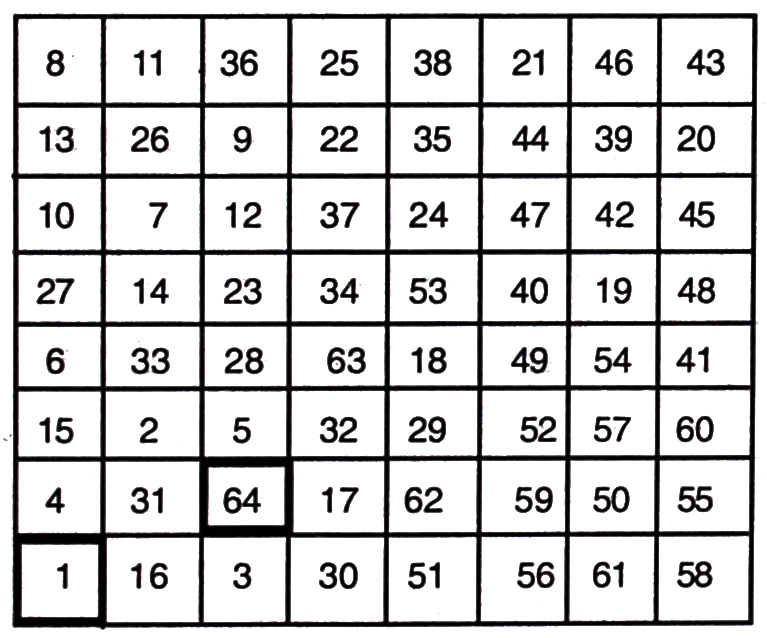
\includegraphics[scale=.9]{src/figures/chap6/fig6-9.jpg}
	\end{figure}
\end{itemize}

\section*{II. 7. $12 \times 12$ ಕುದುರೆ ನಡಿಗೆಯ ಚೌಕ :}

\begin{figure}[H]
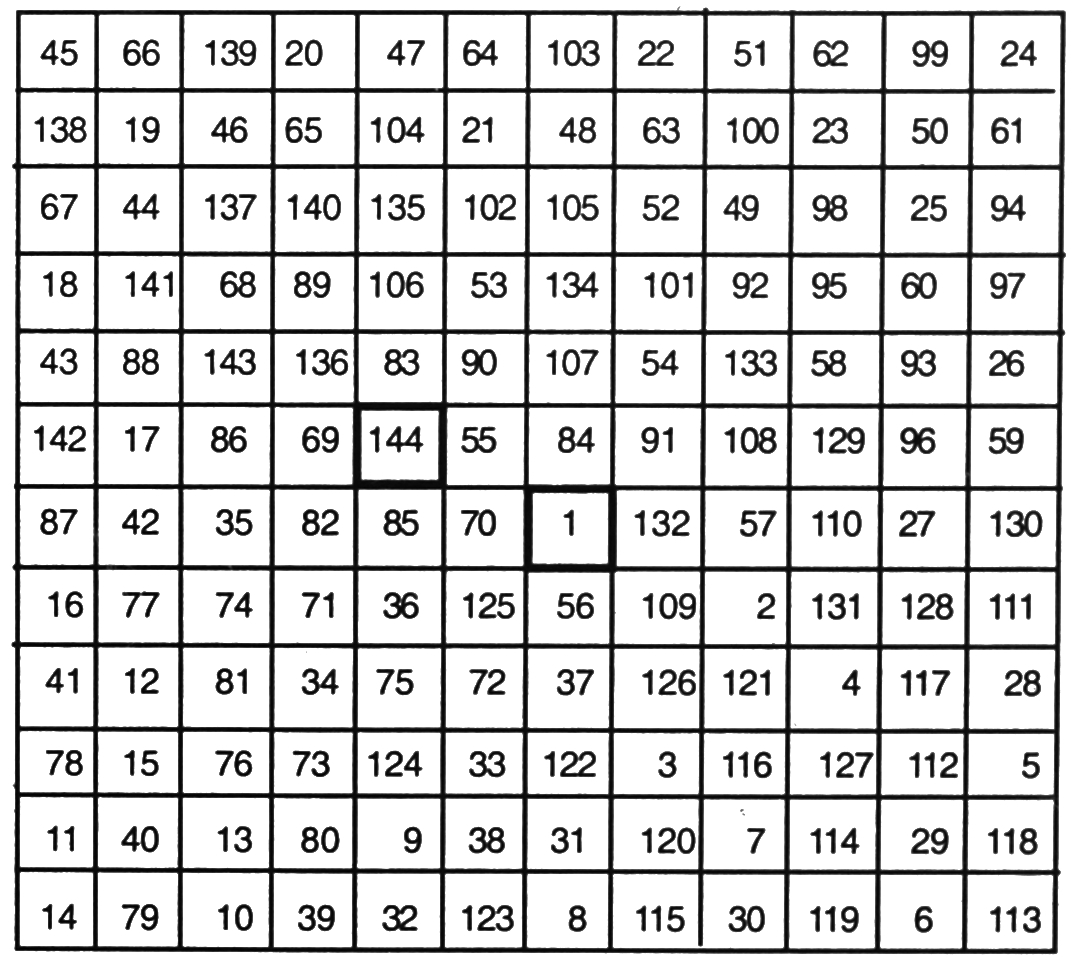
\includegraphics[scale=1.1]{src/figures/chap6/fig6-10.jpg}
\end{figure}
\begin{itemize}
	\item ಮೈಸೂರಿನ ಮಹಾರಾಜರಾಗಿದ್ದ ಮುಮ್ಮಡಿ ಕೃಷ್ಣರಾಜ ಒಡೆಯರ್ (1794-1868) ಅವರು ರಚಿಸಿದ ಗ್ರಂಥ \textbf{‘‘ಚತುರಂಗ ಸಾರಸರ್ವಸ್ವ’’} ದಿಂದ ಆಯ್ಕೆ \smallskip
	\item \textbf{ಮಾಯಾಚೌಕವಲ್ಲ.}\smallskip
	\item 1ರಿಂದ 144 ವರೆಗಿನ ಸಂಖ್ಯೆಗಳನ್ನು ಕುದುರೆ ನಡಿಗೆಯಲ್ಲಿ ಕ್ರಮವಾಗಿ ತುಂಬಿಸಿದೆ.\smallskip
	\item \textbf{‘‘ಮುಚ್ಚಿದ’’} ಅಥವಾ \textbf{‘‘ಪುನಃ ಪ್ರವೇಶ’’} (Re entrant) ಚೌಕ.\smallskip
	\item ಸಂಖ್ಯಾ ಪಲ್ಲಟ ಮಾಡುವುದರಿಂದ 288 ಬೇರೆ ಬೇರೆ ಚೌಕಗಳು ಲಭ್ಯ\smallskip
	\item ಚೌಕವನ್ನು ರಚಿಸುವ ವಿಧಾನವನ್ನು ಸಂಸ್ಕೃತ ಶ್ಲೋಕಗಳ ರೂಪದಲ್ಲಿ ಬರೆಯಲಾಗಿದೆ. ಪದಸಂಖ್ಯೆಗಳನ್ನು ಬಳಸಿ ಶ್ಲೋಕ ರಚನೆ ಇದೆ.
\end{itemize}

\section*{V III. 8. ಪದ್ಯ ಪ್ರದಕ್ಷಿಣಾಬಂಧ ಅಶ್ವಗತಿ ಚಕ್ರ :}

ಇದೂ ಸಹ ಮೈಸೂರಿನ ಅರಸರಾಗಿದ್ದ \textbf{ಮುಮ್ಮಡಿ ಕೃಷ್ಣರಾಜ ಒಡೆಯರ್} ಅವರು ರಚಿಸಿ\-ರುವುದು. ಇದು $12 \times 12$ಚೌಕವಾಗಿದ್ದು, ನಾಲ್ಕು ಮೂಲೆಗಳ $2 \times 2$ಚೌಕಗಳಲ್ಲಿ ಹಾಗೂ ಕೇಂದ್ರದಲ್ಲಿನ $4 \times 4$ಚೌಕದಲ್ಲಿ ಚೌಕವನ್ನು ರಚಿಸಿದವರ ಬಗೆಗೆ ತಿಳಿಸಲಾಗಿದೆ. ಉಳಿದಂತೆ 112 ಮನೆಗಳಲ್ಲಿ (144-32=112) 1ರಿಂದ 112 ವರೆಗಿನ ಸಂಖ್ಯೆಗಳನ್ನು ಕ್ರಮವಾಗಿ ಕುದುರೆ ನಡಿಗೆಯಲ್ಲಿ ತುಂಬಿಸಿದೆ. ಇದು ಮಾಯಾಚೌಕವಲ್ಲ.
\begin{figure}[H]
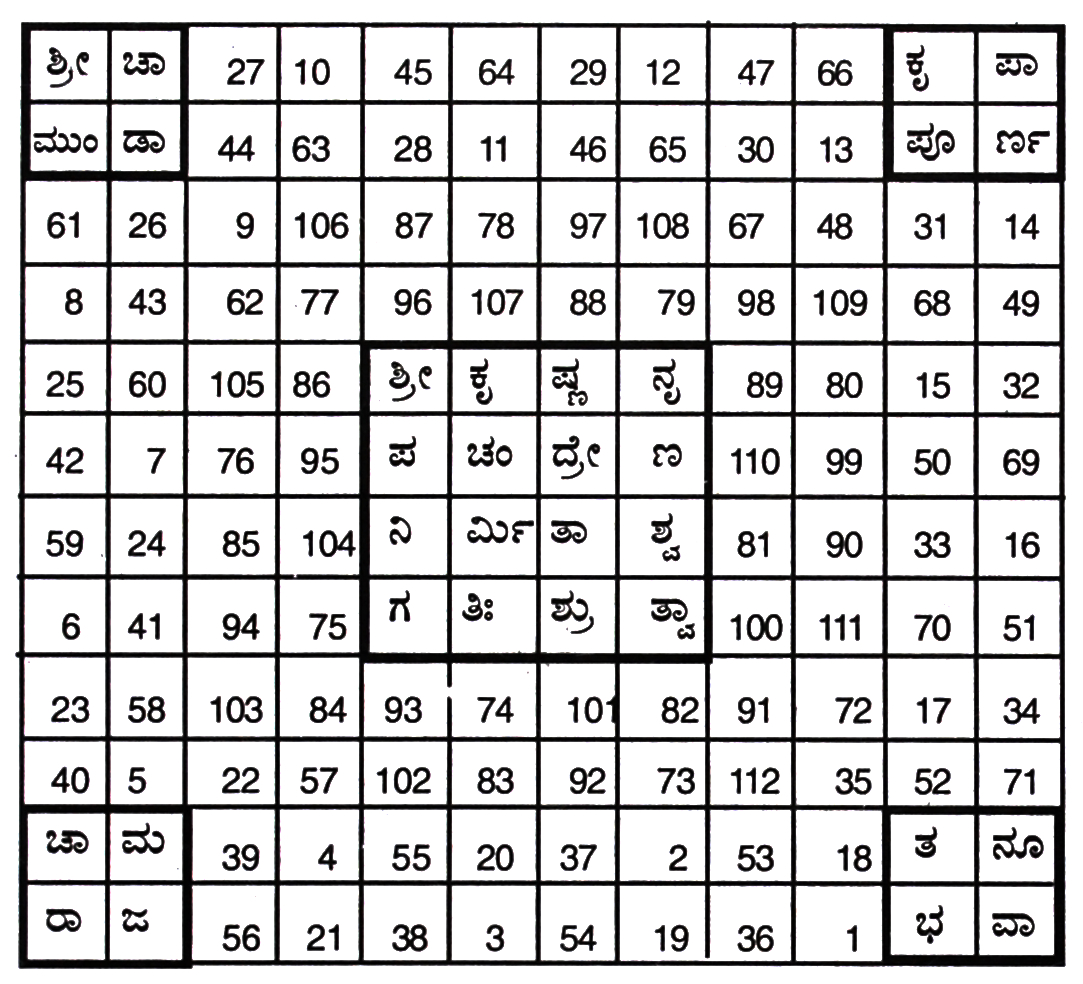
\includegraphics{src/figures/chap6/fig6-11.jpg}
\end{figure}

\begin{itemize}
	\item ಇದು ‘‘ಮುಚ್ಚಿದ’’ ಅಥವಾ ‘‘ಪುನಃಪ್ರವೇಶ’’ ಚೌಕ.
	\item \textbf{ಶ್ಲೋಕ ಹೀಗಿದೆ :}
	\begin{quote}
	ಶ್ರೀಚಾಮುಂಡಾ ಕೃಪಾಪೂರ್ಣ ಚಾಮರಾಜ ತನೂಭವಾ ।\\
	ಶ್ರೀ ಕೃಷ್ಣನೃಪ ಚಂದ್ರೇಣ ನಿರ್ಮಿತಾಶ್ವ ಗತಿಃ ಶ್ರುತ್ವಾ ॥
	\end{quote}
\end{itemize}

\textbf{ಅರ್ಥ :} ಶ್ರೀ ಚಾಮುಂಡೇಶ್ವರಿ ಕೃಪಾ ಪೋಷಿತರಾದ ಚಾಮರಾಜ ಒಡೆಯರ ಪುತ್ರರಾದ ಶ್ರೀಕೃಷ್ಣರಾಜ ಒಡೆಯರಿಂದ ರಚಿತವಾದ ಅಶ್ವಗತಿ ಚೌಕ.

\section*{V III. 9. $12 \times 12$ ರ ಮಾಯಾ ಚಿತ್ರ :}
\begin{figure}[H]
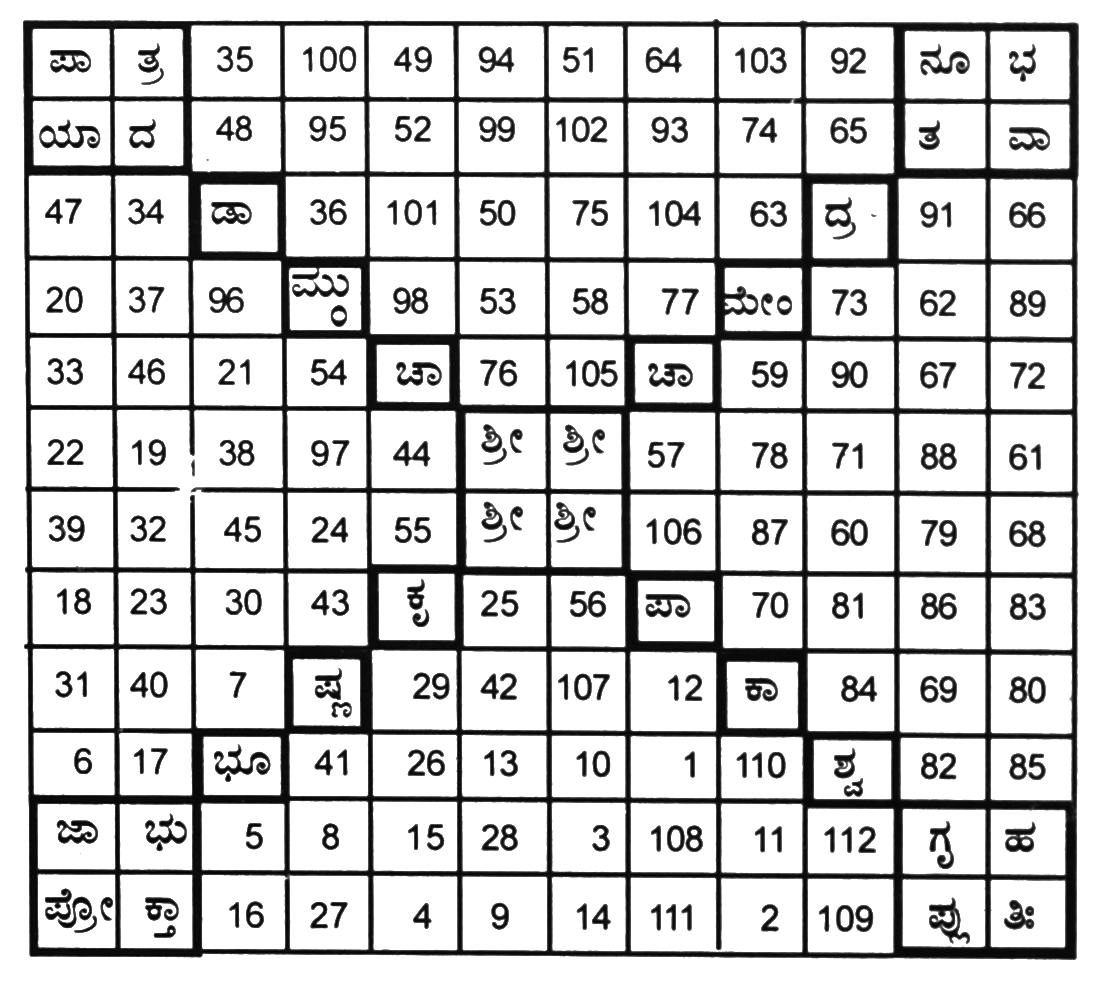
\includegraphics{src/figures/chap6/fig6-12.jpg}
\end{figure}

\begin{itemize}
	\item ಮೈಸೂರಿನ ಮಹಾರಾಜರಾಗಿದ್ದ ಮುಮ್ಮಡಿ ಕೃಷ್ಣರಾಜ ಒಡೆಯರ್ (1794-1868) ಅವರ ರಚನೆ.
	\item ಮಾಯಾ ಚೌಕವಲ್ಲ.
	\item $12 \times 12$ ಚೌಕದ 144 ಮನೆಗಳಲ್ಲಿ 32 ಮನೆಗಳಲ್ಲಿ ಶ್ಲೋಕಾಕ್ಷರಗಳಿವೆ.
	\item ಉಳಿದ 112 ಮನೆಗಳಲ್ಲಿ 1ರಿಂದ 112 ರವರೆಗೆ ಸಂಖ್ಯೆಗಳನ್ನು ಕುದುರೆ ನಡಿಗೆಯಲ್ಲಿ ತುಂಬಿಸಿದೆ.
	\item ತೆರೆದ ಚೌಕ
	\item \textbf{ಶ್ಲೋಕ :} 
	\begin{quote}
	ಶ್ರೀಚಾಮುಂಡಾ ದಯಾಪಾತ್ರ ಶ್ರೀಚಾಮೇಂದ್ರ ತನೂಭವಾ ।\\
	ಶ್ರೀಕೃಷ್ಣ ಭೂಭುಚಾಪ್ರೋಕ್ತಾ ಶ್ರೀಪಾಕಾಶ್ವಗೃಹ ಪ್ಲುತಿಃ ॥
	\end{quote}
	ಚೌಕದ ಮಧ್ಯದಿಂದ ತೊಡಗಿ ಕರ್ಣಗಳಲ್ಲಿ ಚಲಿಸಿ, ಓದಿ.
\end{itemize}

\section*{ III. 10.}

\begin{figure}[H]
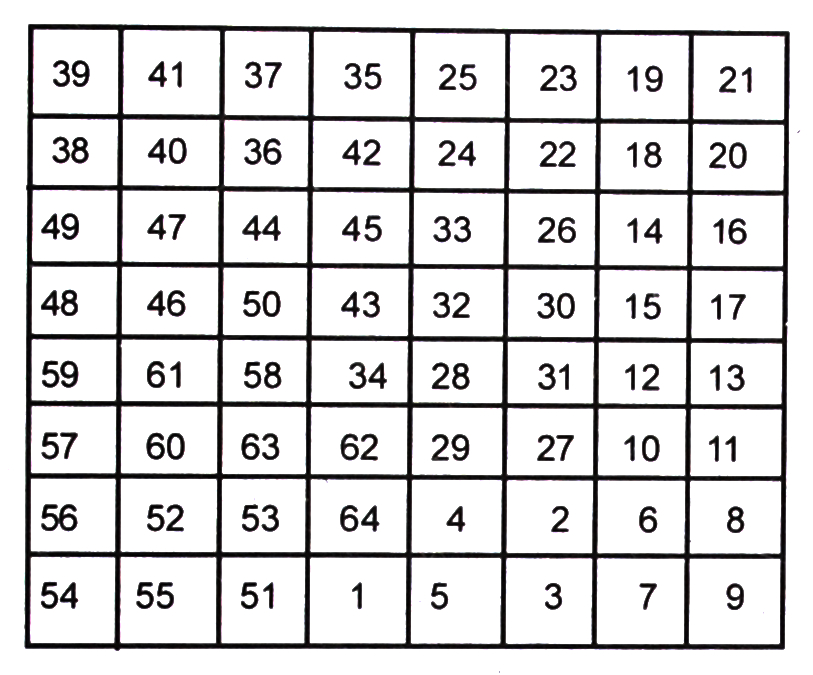
\includegraphics{src/figures/chap6/fig6-13.jpg}
\end{figure}

ಕುದುರೆ, ಆನೆ, ಮಂತ್ರಿ ರಾಜ - ಇವುಗಳ ನಡಿಗೆ. ಪರ್ಯಾಯವಾಗಿ ಅದೇ ಕ್ರಮದಲ್ಲಿದೆ. 1 ರಿಂದ 64 ಕ್ರಮಾಗತ ಸಂಖ್ಯೆಗಳು. ಆನೆ ನಡಿಗೆಯಲ್ಲಿ ಕೆಲವೊಮ್ಮೆ 1 ಕ್ಕಿಂತ ಹೆಚ್ಚು ಮನೆಗಳನ್ನು ಕ್ರಮಿಸಿದೆ. 26 ರಿಂದ 27, 34-35, 50-51ಇತ್ಯಾದಿ ಗಮನಿಸಿ.
\begin{figure}[H]
\includegraphics{src/figures/chap6/fig6-14.eps}
\end{figure}

ಮಧ್ಯದಲ್ಲಿ ಮಸುಕುಮಾಡಿರುವ 12 ಮನೆಗಳನ್ನು ಕುದುರೆ ನಡಿಗೆಯಲ್ಲಿ ಮೊದಲು \hbox{ತುಂಬಿಸಿ ನಂತರ} ಉಳಿದ ಮನೆಗಳನ್ನು ಕುದುರೆ ನಡಿಗೆಯಲ್ಲಿ ತುಂಬಿಸಿದೆ. 1 ರಿಂದ 64 ಕ್ರಮಾ\-ಗತ ಸಂಖ್ಯೆಗಳು.

\begin{figure}[H]
\includegraphics[scale=.95]{src/figures/chap6/fig6-15.eps}
\end{figure}
ಆರನೆ ಅಡ್ಡಸಾಲಿನಲ್ಲಿ 3ರ ಗುಣಕಗಳನ್ನು ಬಲದಿಂದ ಎಡಕ್ಕೆ ತುಂಬಿಸಿದೆ. ಎಲ್ಲ ಮನೆ\-ಗಳನ್ನೂ ಕುದುರೆ ನಡಿಗೆಯಲ್ಲಿ ತುಂಬಿಸಿದೆ. 1ರಿಂದ 64 ಕ್ರಮಾಗತ ಸಂಖ್ಯೆಗಳು.
\begin{figure}[H]
\includegraphics[scale=.95]{src/figures/chap6/fig6-16.eps}
\end{figure}
4ನೆ ಅಡ್ಡಸಾಲಿನಲ್ಲಿ 26ರಿಂದ ಪ್ರಾರಂಭಿಸಿ 5 ಹೆಚ್ಚಿಸುತ್ತಾ, ಬಲದಿಂದ ಎಡಕ್ಕೆ ತುಂಬಿಸಿದೆ. 6ನೆ ಅಡ್ಡಸಾಲಿನಲ್ಲಿ, 1ರಿಂದ ಷುರುಮಾಡಿ 3 ಹೆಚ್ಚಿಸುತ್ತಾ ಎಡದಿಂದ ಬಲಕ್ಕೆ ತುಂಬಿಸಿದೆ. ಎಲ್ಲ ಮನೆಗಳೂ ಕುದುರೆ ನಡಿಗೆಯಲ್ಲಿ ತುಂಬಲ್ಪಟ್ಟಿವೆ. 1ರಿಂದ 64 ಕ್ರಮಾಗತ ಸಂಖ್ಯೆಗಳು.
\begin{figure}[H]
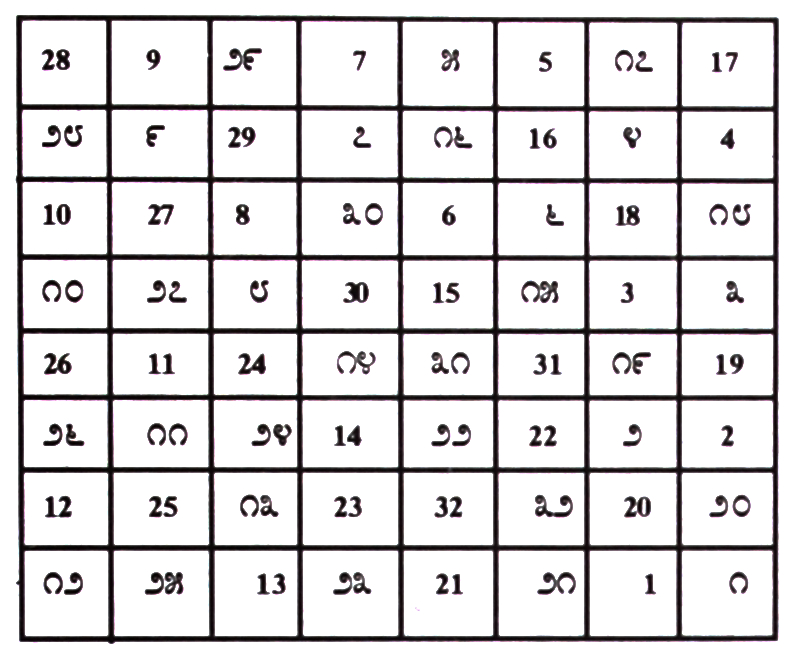
\includegraphics[scale=1.1]{src/figures/chap6/fig6-17.jpg}
\end{figure}

ಎರಡು ಕುದುರೆಗಳ ನಡಿಗೆಯಿಂದ ಎಲ್ಲ ಮನೆಗಳನ್ನು ತುಂಬಿಸಿದೆ. ವ್ಯತ್ಯಾಸ ತಿಳಿಯಲು ಹಿಂದೂ ಅರಾಬಿಕ್ ಮತ್ತು ಕನ್ನಡ ಸಂಖ್ಯೆ ಬಳಸಿದೆ. 1ರಿಂದ 32 ಕ್ರಮಾಗತ ಸಂಖ್ಯೆಗಳು.
\begin{figure}[H]
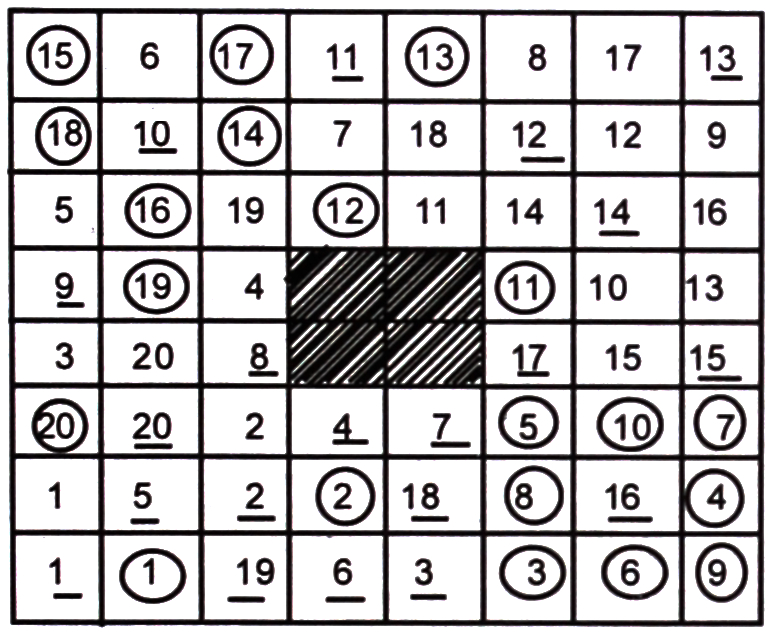
\includegraphics[scale=1.1]{src/figures/chap6/fig6-18.jpg}
\end{figure}

ಮಧ್ಯದ 4 ಮನೆಗಳನ್ನು ಹೊರತುಪಡಿಸಿ ಉಳಿದ 60 ಮನೆಗಳನ್ನು 3 ಕುದುರೆಗಳ ನಡಿಗೆಯಿಂದ ತುಂಬಿಸಿದೆ. ಪ್ರತಿ ಕುದುರೆಯೂ 1 ರಿಂದ 20 ಮನೆಗಳಿಗೆ ಚಲಿಸಿದೆ. ಮೂರು ಕುದುರೆ\-ಗಳನ್ನು ಗುರುತಿಸಲು ಅನುಕೂಲವಾಗುವಂತೆ ಒಂದನ್ನು ವೃತ್ತೀಕರಿಸಿದೆ. ಇನ್ನೊಂದಕ್ಕೆ ತಳಗೆರೆ (Underline) ಎಳೆದಿದೆ. ಮತ್ತೊಂದು ಹಾಗೆಯೇ ಇದೆ.

ನಾಲ್ಕು ಕುದುರೆಗಳ ನಡಿಗೆಯಲ್ಲಿ ಎಲ್ಲಾ 64 ಮನೆಗಳನ್ನು ತುಂಬಿಸಿದೆ. 1ರಿಂದ 16 ಕ್ರಮಾಗತ ಸಂಖ್ಯೆಗಳು. ಒಂದನ್ನು ವೃತ್ತೀಕರಿಸಿದೆ. ಒಂದಕ್ಕೆ ಒಂದು ತಳಗೆರೆ, ಇನ್ನೊಂದಕ್ಕೆ 2 ತಳಗೆರೆ ಹಾಕಿದೆ. ಮತ್ತೊಂದು ಹಾಗೆಯೇ ಇದೆ.
\begin{figure}[H]
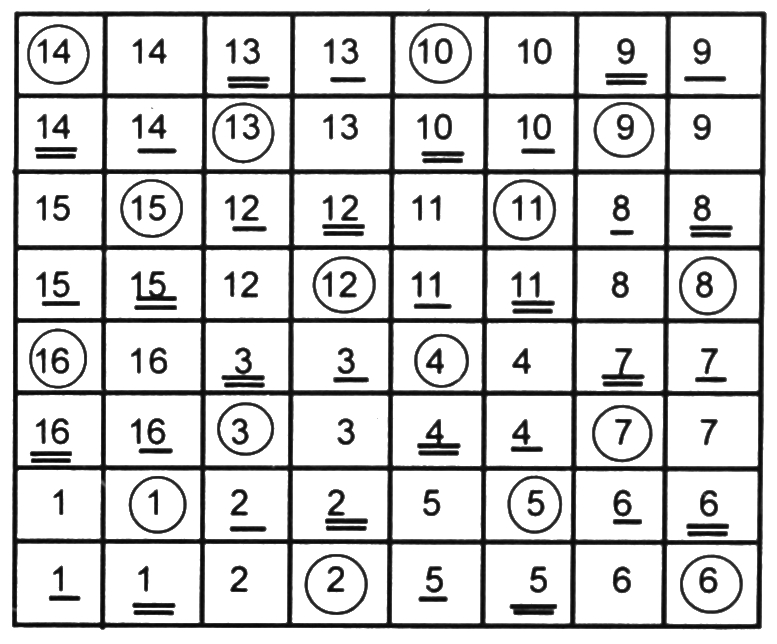
\includegraphics[scale=.88]{src/figures/chap6/fig6-19.jpg}
\end{figure}

64 ಮನೆಗಳಲ್ಲಿ ಮಧ್ಯದಲ್ಲಿ 8 ಮನೆಗಳನ್ನು ಮಸುಕು ಮಾಡಿದೆ. (Shaded) 5ರ ಗುಣಕ\-ಗಳಿಂದ ತುಂಬಿಸಿದೆ. ಎಲ್ಲ 64 ಮನೆಗಳನ್ನು ಕುದುರೆ ನಡಿಗೆಯಿಂದ ತುಂಬಿಸಿದೆ. 1ರಿಂದ 64ವರೆಗೆ ಕ್ರಮಾಗತ. ಸಂಖ್ಯೆಗಳು. ತೆರೆದ ಚೌಕ.
\begin{figure}[H]
\includegraphics[scale=.78]{src/figures/chap6/fig6-20.eps}
\end{figure}

ಒಂದು ಕರ್ಣ 8ರ ಗುಣಕಗಳು

ಅಶ್ವಗತಿ ಬಂಧ

1 ರಿಂದ 64 ಕ್ರಮಾಗತ ಸಂಖ್ಯೆಗಳು.
\begin{figure}[H]
\includegraphics[scale=.9]{src/figures/chap6/fig6-21.eps}
\end{figure}
\begin{figure}[H]
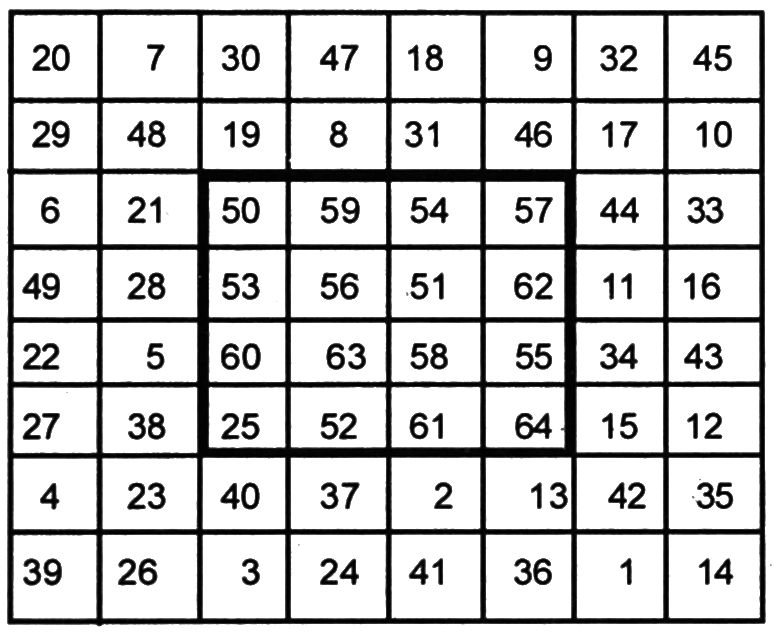
\includegraphics[scale=.95]{src/figures/chap6/fig6-22.jpg}
\end{figure}

ಪ್ರದಕ್ಷಿಣ ಅಪ್ರದಕ್ಷಿಣ ಅಶ್ವಗತಿ ಬಂಧ 1ರಿಂದ 64 ಕ್ರಮಾಗತ ಸಂಖ್ಯೆಗಳು

ಕುದುರೆ ಮತ್ತು ಮಂತ್ರಿ (Queen) ಗಳ ಪರ್ಯಾಯ ನಡಿಗೆಯಿಂದ ತುಂಬಿಸಿದೆ. 1ರಿಂದ 64 ಕ್ರಮಾಗತ ಸಂಖ್ಯೆಗಳು. ಮಂತ್ರಿ ನಡಿಗೆಯನ್ನು ಓರೆ ಗೆರೆ ( {\textbackslash ,} / ) ಯಿಂದ ಸೂಚಿಸಿದೆ.
\begin{figure}[H]
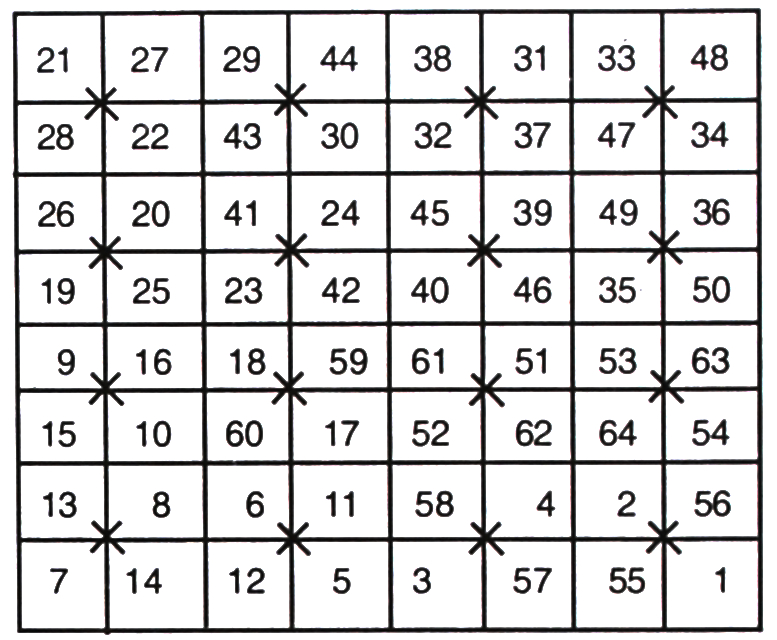
\includegraphics{src/figures/chap6/fig6-23.jpg}
\end{figure}

ಕುದುರೆ ಮತ್ತು ಒಂಟೆ (ರಥ, Bishop) ಪರ್ಯಾಯ ನಡಿಗೆಯಿಂದ ತುಂಬಿಸಿದೆ. 1ರಿಂದ 64 ಕ್ರಮಾಗತ ಸಂಖ್ಯೆಗಳು. ಒಂಟೆ ನಡಿಗೆಯಲ್ಲಿ ಕೆಲವನ್ನು ಓರೆ ಗೆರೆಗಳಿಂದ ಸೂಚಿಸಿದೆ.
\begin{figure}[H]
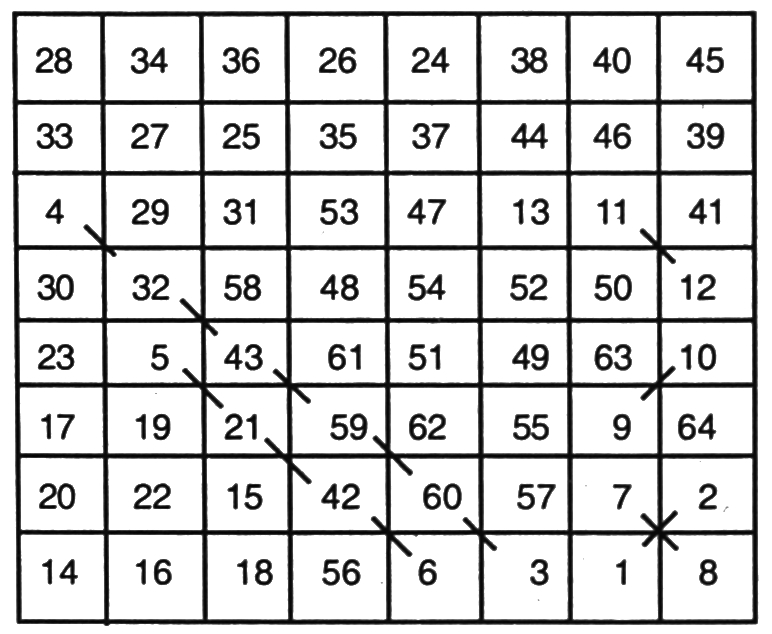
\includegraphics{src/figures/chap6/fig6-24.jpg}
\end{figure}

ಒಂಟೆ ಚಲನೆಯಲ್ಲಿ ಒಂದು ನಡಿಗೆಯಲ್ಲಿ ಕೆಲವು ಮನೆಗಳನ್ನು ಹಾದು ಹೋಗಿದೆ. ನೋಡಿ 13-14, 23-24, 17-18.
